\documentclass[10pt]{article}
\usepackage{graphicx}
\usepackage[none]{hyphenat}
\usepackage{graphicx}
\usepackage{listings}
\usepackage[english]{babel}
\usepackage{siunitx}
\usepackage{graphicx}
\usepackage{caption} 
\usepackage{booktabs}
\usepackage{array}
\usepackage{amssymb} % for \because
\usepackage{amsmath}   % for having text in math mode
\usepackage{extarrows} % for Row operations arrows
\usepackage{listings}
\usepackage[utf8]{inputenc}
\lstset{
  frame=single,
  breaklines=true
}
\usepackage{hyperref}
  
%Following 2 lines were added to remove the blank page at the beginning
\usepackage{atbegshi}% http://ctan.org/pkg/atbegshi
\AtBeginDocument{\AtBeginShipoutNext{\AtBeginShipoutDiscard}}


%New macro definitions
\newcommand{\mydet}[1]{\ensuremath{\begin{vmatrix}#1\end{vmatrix}}}
\providecommand{\brak}[1]{\ensuremath{\left(#1\right)}}
\newcommand{\solution}{\noindent \textbf{Solution: }}
\newcommand{\myvec}[1]{\ensuremath{\begin{pmatrix}#1\end{pmatrix}}}
\providecommand{\norm}[1]{\left\lVert#1\right\rVert}
\providecommand{\abs}[1]{\left\vert#1\right\vert}
\let\vec\mathbf{}
\begin{document}

\begin{center}
\title{\textbf{LINES}}
\date{\vspace{-5ex}} %Not to print date automatically
\maketitle
\end{center}

\section*{11$^{th}$ Maths - EXERCISE-10.4}

Find the  equations of the lines, which cutoff intercepts on the axes  whose sum and product are 1 and -6 respectively.

\solution
Let the intercepts of $x$ and $y$ are $a$ and $b$\\
Given
\begin{align}
a+b&=1
\label{eq1}\\
ab&=-6
\label{eq2}
\end{align} 
on solving \eqref{eq1} and \eqref{eq2} we get\\
$$\implies a=3,b=-2 \text{ or }   a=-2,b=3$$\\

Thus,the possible intercepts are\\
\begin{align}
\vec{a}&=\myvec{3\\0},\vec{b}=\myvec{0\\-2}\\
\vec{c}&=\myvec{-2\\0},\vec{d}=\myvec{0\\3}
\end{align}
\begin{align}
\vec{m}&=\vec{a}-\vec{b}\\
&=\myvec{3\\0}-\myvec{0\\-2}\\
&=\myvec{3\\2}\\
\vec{m}&=\myvec{3\\2} \text{or,} \myvec{-2\\-3}
\end{align}
\begin{enumerate}
\item For\\
\begin{align}
\vec{n} = \myvec{ 2\\-3}\\
\end{align}
the equation of the line will be\\
\begin{align}
\vec{n}^{\top}\brak{\vec{x}-\vec{A}}&=0\\
\myvec{2&-3}\vec{x}&=-6
\end{align}
\item For\\
\begin{align}
\vec{n}=\myvec{-3\\2}\\
\end{align}
the equation of the line will be\\
\begin{align}
\vec{n}^{\top}\brak{\vec{x}-\vec{B}}&=0\\
\myvec{-3&2}\vec{x}&=-6
\end{align}
\end{enumerate}
\begin{figure}[!h]
	\begin{center}
		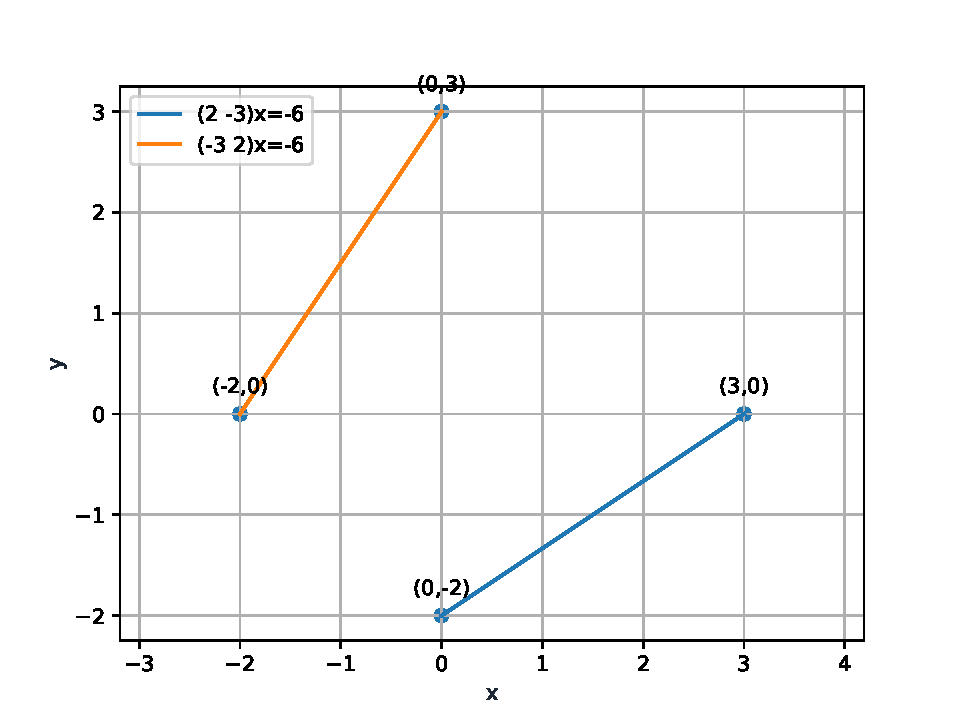
\includegraphics[width=\columnwidth]{./figs/fig.pdf}
	\end{center}
\caption{}
\label{figure}
\end{figure}
\end{document}
